\newpage
\thispagestyle{empty}
\chapter{PROJECT WORK}
\section{Adding support to persistent storage}

As I already mentioned in the section \ref{swtraining}, Software training, that we were having an issue with the old setup of the \textit{SNARE \& TANNER}. 
\begin{figure}[h!]
    \centering  
    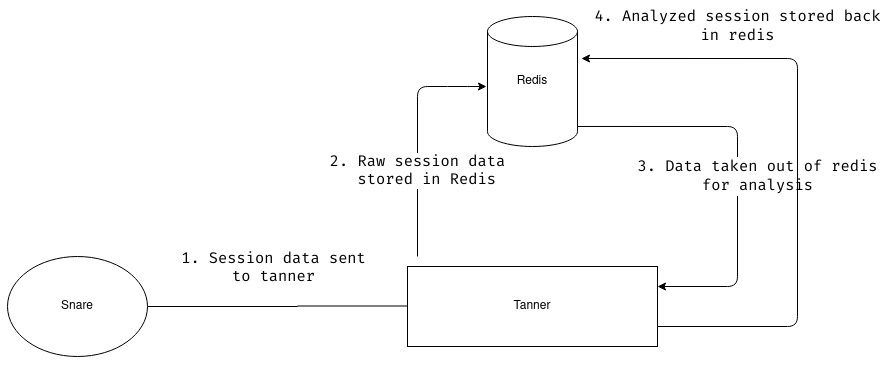
\includegraphics[width=.9\textwidth]{old-setup}
    \caption{old honeypot setup}
    \label{fig:1}
\end{figure}
\subsection{Disadvantages of this setup}
As mentioned above higher consumption of memory on a low spec system would result in an unexpected crash of TANNER server. Also, higher memory consumption would cause other memory issues like slowing down other applications present on the system.
\subsection{The Solution}
First, we decided that we can add support for Postgres, and then we'll give users the option to run tanner either with Redis or with Postgres. But later after some discussion, we decided that we'll use a combination of Redis and Postgres.

The way we decided to use them can be seen in the following diagram:
\begin{figure}[h!]
    \centering
    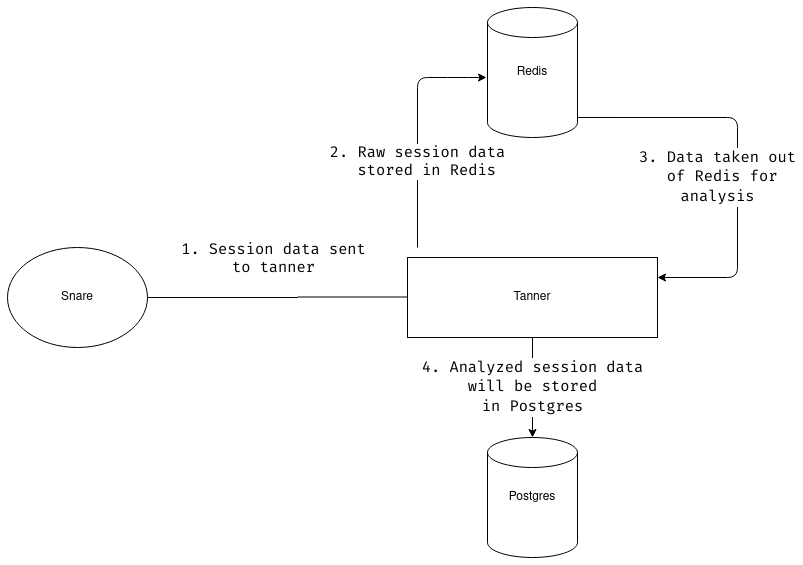
\includegraphics[width=.9\textwidth]{new-setup}
    \caption{New honeypot Setup}
    \label{fig:2}
\end{figure}
As it's clear from the above diagram that after analysis we are storing the data in the Postgres and then we are deleting the analyzed data from Redis.

The advantages of using the combination of both Postgres and Redis are
\begin{itemize}
    \item When TANNER receives a session from SNARE it will be able to store that session data in Redis with much higher speed.

    \item Once the session is analyzed then it can be stored in persistent disk storage like Postgres.
\end{itemize}
\section{Change in Data format}
One of the major advantages of having Postgres as the storage is because it gives us the power to perform queries before presenting that data to the user.

TANNER API is used to access the data stored in the DB. Let's take an example to understand how the API has changed now, we have an endpoint /snare-stats/<snare-uuid> which returns stats like Number of attacks, total sessions, etc of a given snare instance.

Now in the old (Only Redis) setup, we were extracting all the data from the DB, and then we were selecting only those keys that were required for that endpoint. But now with the new (Redis+Postgres) setup, we don't extract all the data. What we do is we run SQL queries on the data before actually extracting the data, this saves us from unnecessary processing.

If you’d like to see the queries we are executing then please check out the code \href{https://github.com/mushorg/tanner/blob/develop/tanner/api/api.py#L49}{here}
\subsection{Detail about the format}
We decided to store all the data in 4 tables named sessions, cookies, owners, paths. If you'd like to see the initial discussion about this format then check out this small \href{https://gist.github.com/mzfr/e7cb772a6c452a12c75230430260022b}{gist} that I made.

Below you can see the schema of all the tables:

\begin{figure}[h!]
    \centering
    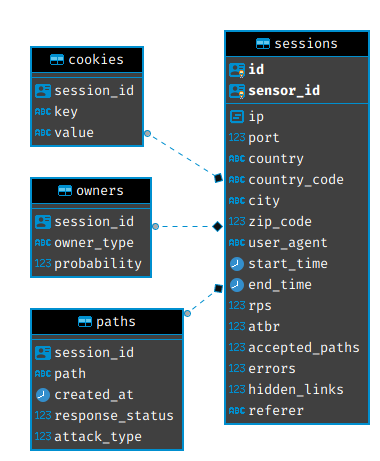
\includegraphics[width=.5\textwidth]{table}
    \caption{DB table Schema}
    \label{fig:3}
\end{figure}
\vfill